\ylDisplay{Polüspast} % Ülesande nimi
{Mihkel Rähn} % Autor
{lõppvoor} % Voor
{2014} % Aasta
{G 6} % Ülesande nr.
{6} % Raskustase
{
% Teema: Staatika
\ifStatement
Jäälõhesse kukkunud alpinisti väljatõmbamiseks on käepärastest vahenditest (kolm plokki ja nöörijupid) koostatud polüspast. Lihtsustatud joonisel on jämeda joonega märgitud põhiköis, mille ühes otsas on kukkunu ning teisest otsast vinnatakse. Plokid on peene joonega kujutatud nööri abil kinnitatud mittelibiseva sõlmega (joonisel täidetud ring) põhiköie külge. Leidke polüspasti ülekandetegur nii hõõrdumist arvestamata kui ka eeldusel, et hõõrdumine vähendab jõuülekannet igal plokil $35\percent$. Eeldage, et kõik jõud on vertikaalsed.

\begin{center}
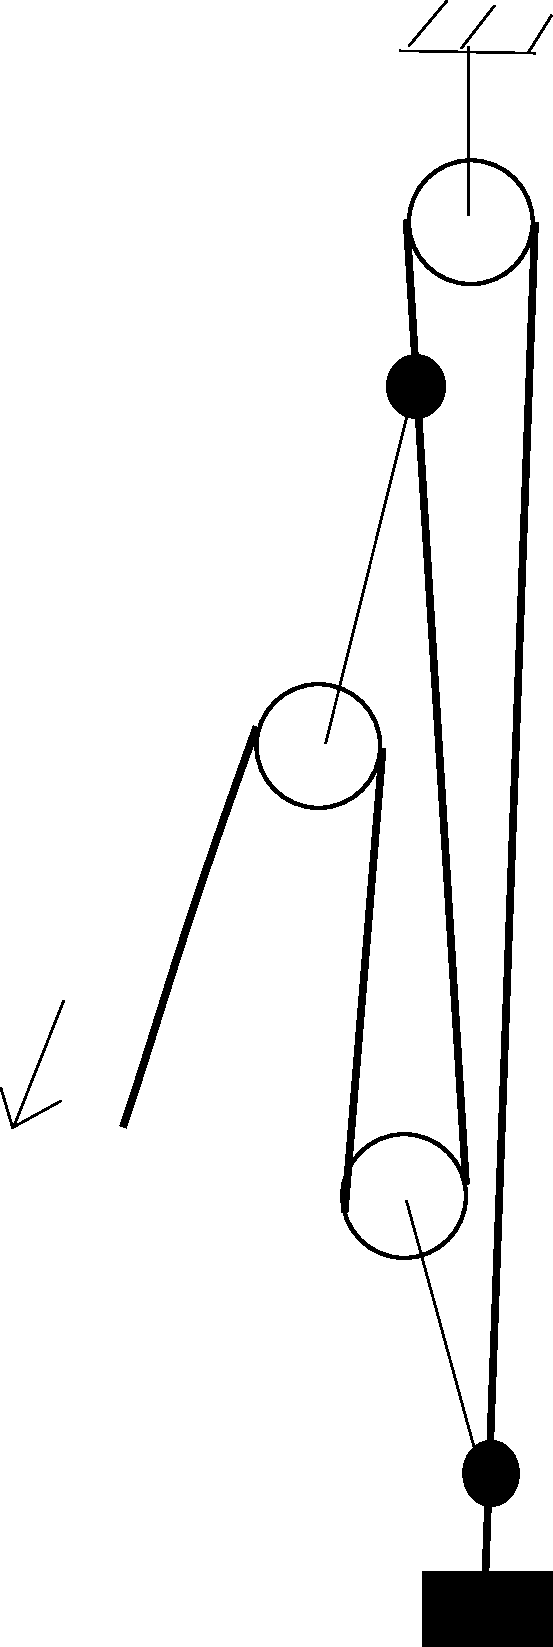
\includegraphics[width=0.25\linewidth]{2014-v3g-06-Polyspast}
\end{center}
\fi


\ifHint
Hõõrdevaba ploki korral on pinge põhiköies jääv, muutub vaid selle suund. Lisaks peab tasakaalutingimuse rahuldamiseks ploki kinnituse pinge olema võrdne plokki läbiva põhiköie pingete summaga. Lahendamise jaoks on mugav alustada päästja poolsest otsast ning öelda, et vastav tõmbejõud on $F$.
\fi


\ifSolution
Hõõrdevaba ploki korral on pinge põhiköies jääv, muutub vaid selle suund. Hõõrdega ploki korral osa põhiköie pingest kandub plokile, kusjuures esmases lähenduses alla ja ülesse suunatud hõõrdejõud kompenseerivad üksteist. Tasakaalutingimuse rahuldamiseks peab ploki kinnituse pinge olema võrdne plokki läbiva põhiköie pingete summaga. Mittelibisevate sõlmede korral peab alla ja üles suunatud pingete vahel valitsema tasakaal. Lahendamist on mugav alustada, kui määrata päästjapoolseks tõmbejõuks $F$ ning alustada sellest otsast polüspasti läbimist. Hõõrdevabal juhul on jõuülekanne $\frac{5}{1}$, hõõrde korral $\frac{\num{2,4}}{1}$.

\begin{center}
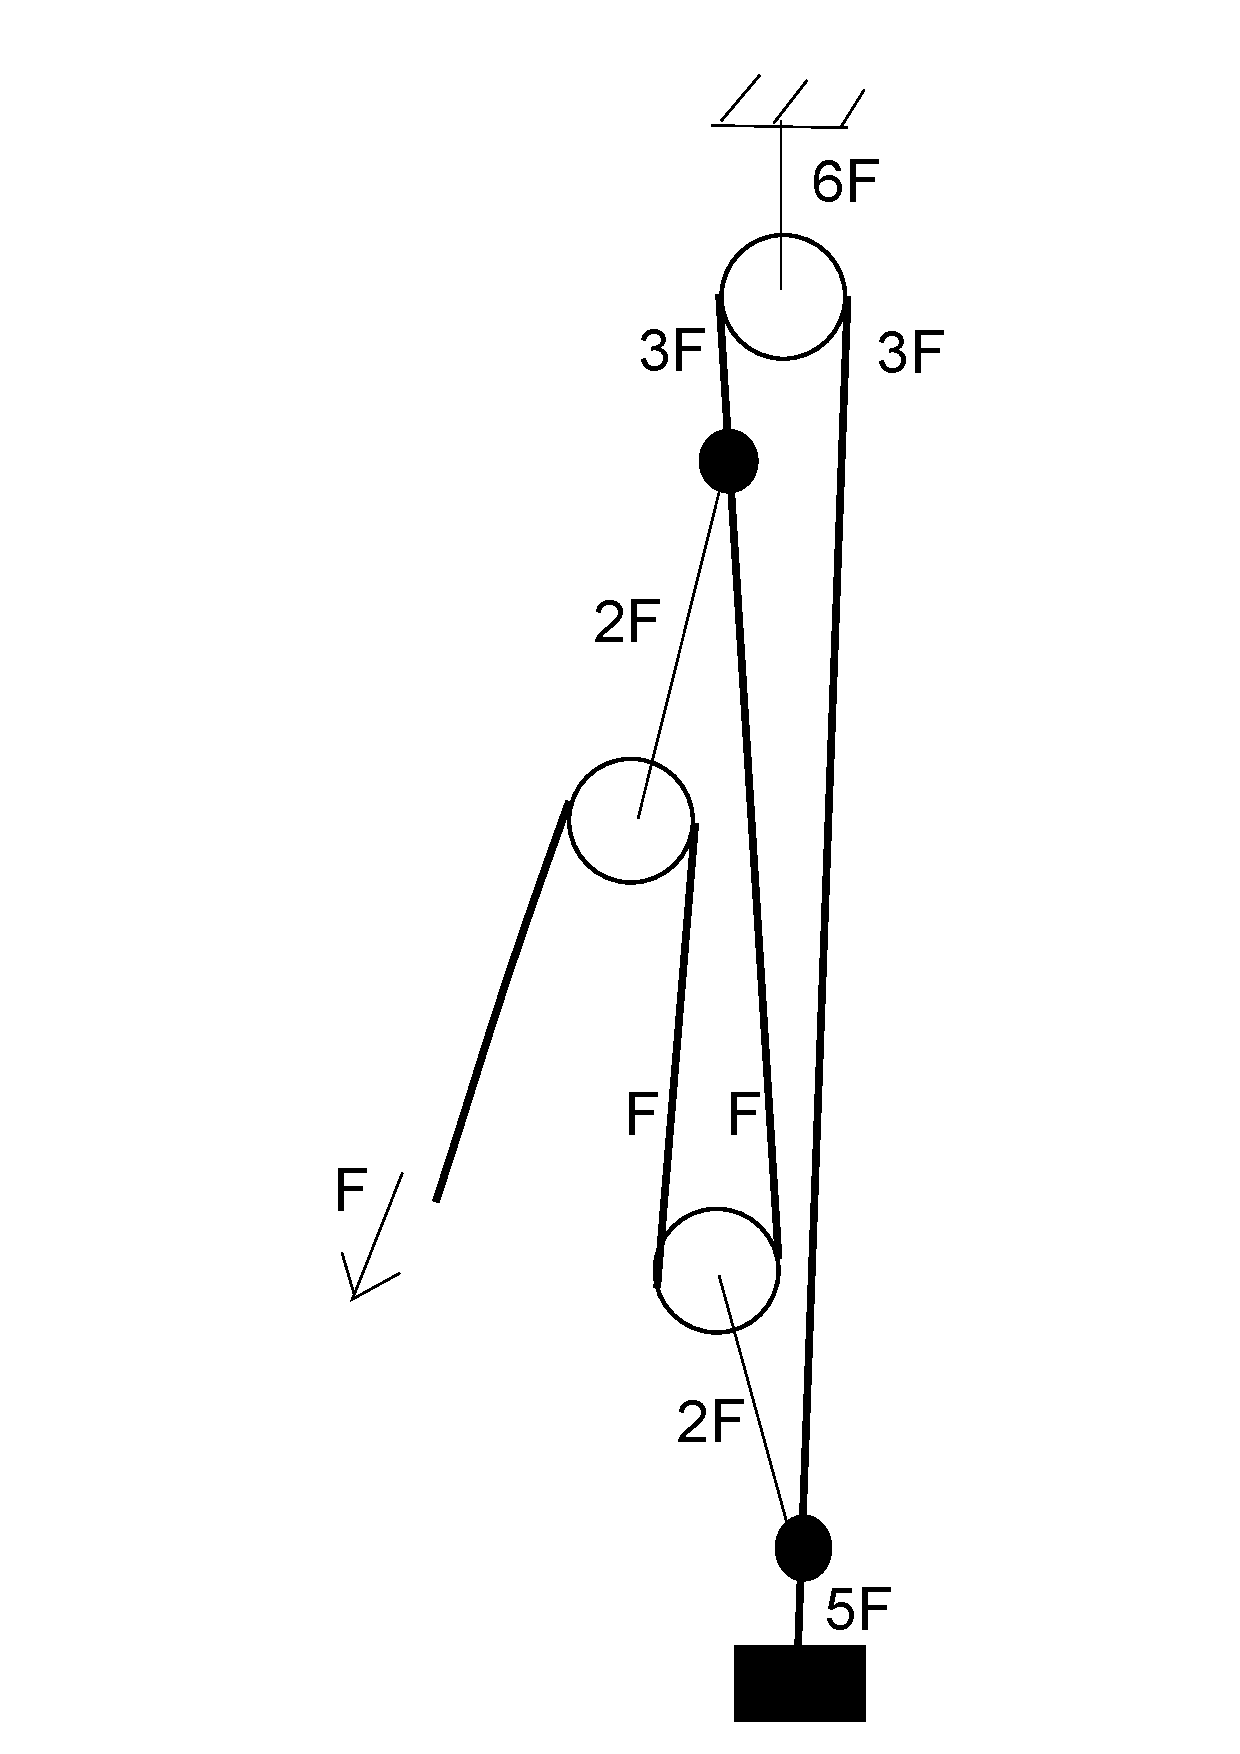
\includegraphics[scale=0.25]{2014-v3g-06-PolyspastL1}
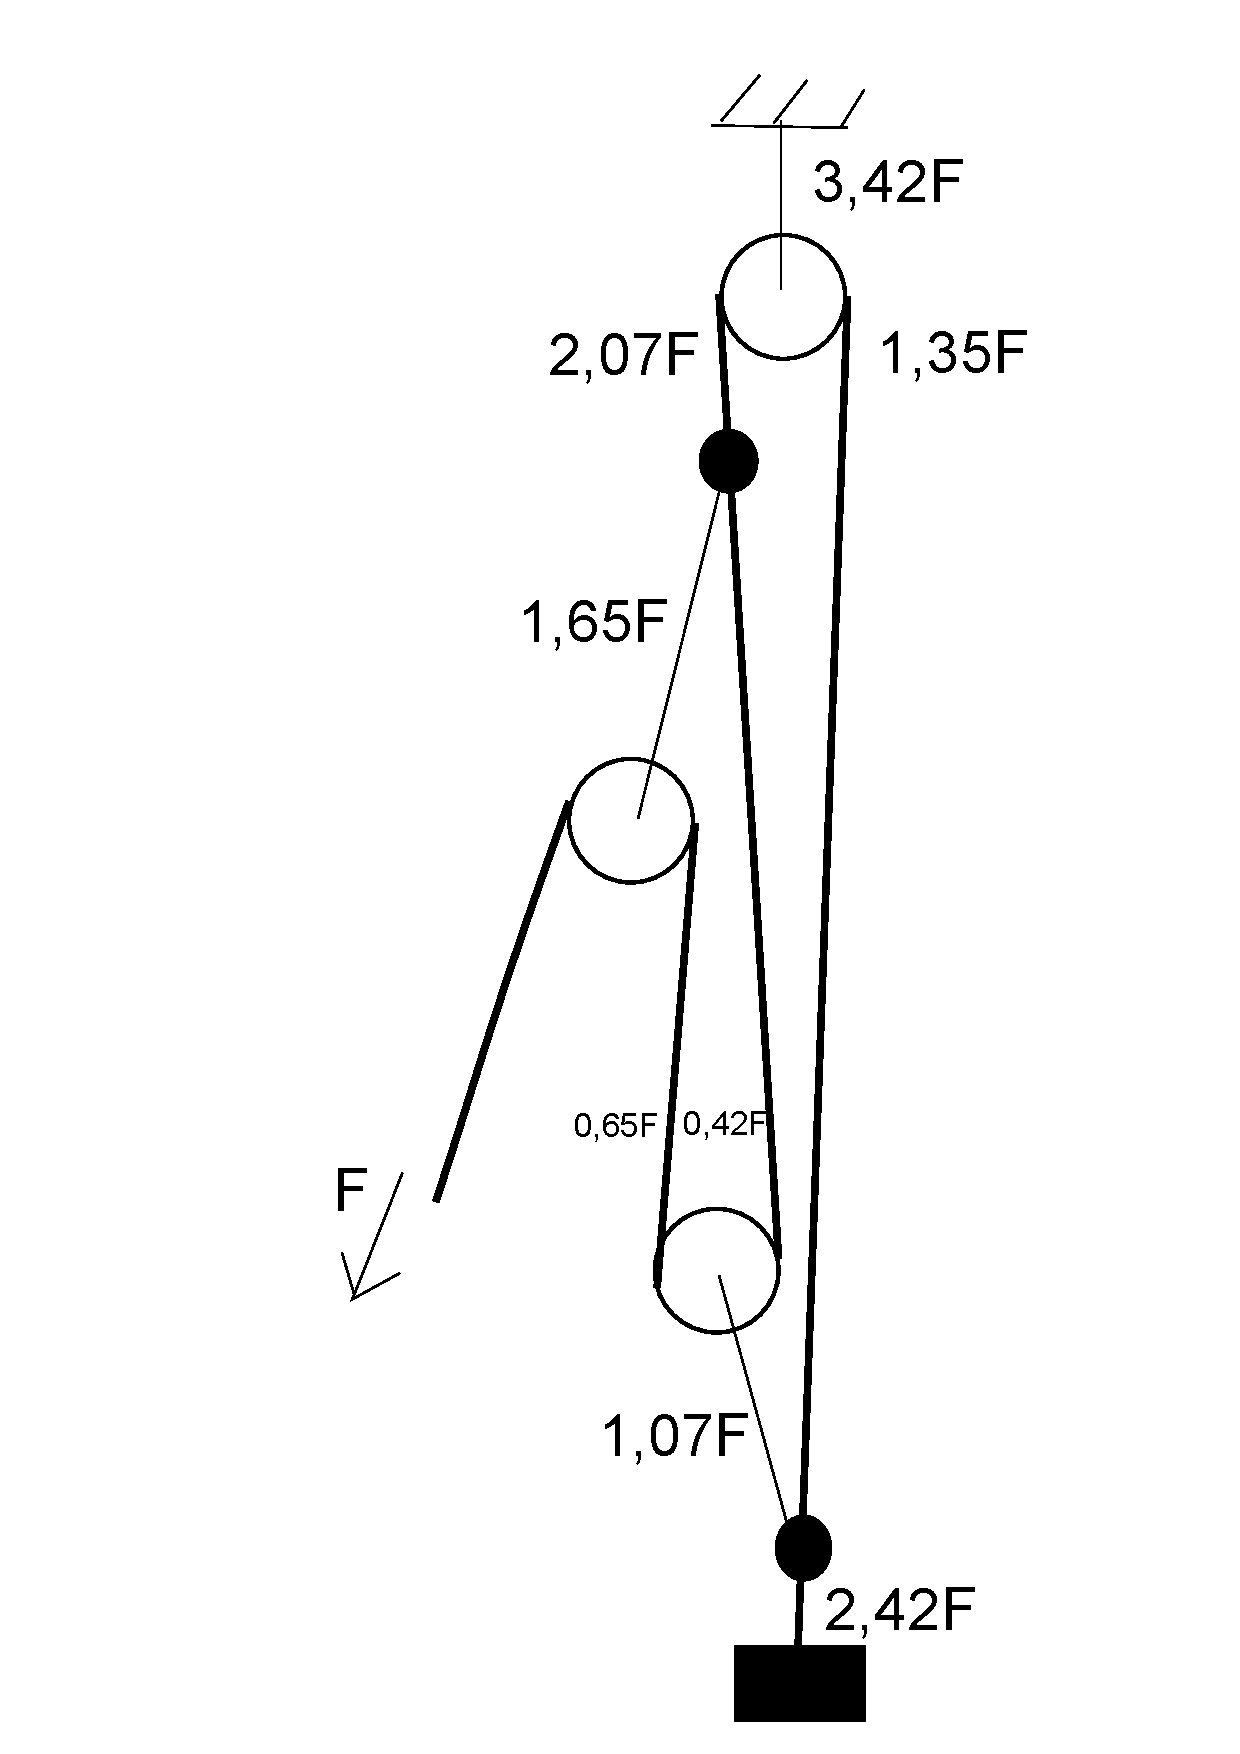
\includegraphics[scale=0.25]{2014-v3g-06-PolyspastL2}
\end{center}
\fi


\ifEngStatement
% Problem name: Polyspast
A polyspast is made from convenient tools (three blocks and parts of rope) to pull out an alpinist who fell into an ice gap. The main rope is marked with a thick line in the simplified figure, the fallen alpinist is attached to one end and the other end is pulled at. The blocks are attached to the main rope with a non-sliding knot with the help of ropes that are depicted as thin lines in the figure. Find the transmission factor of the polyspast while not accounting for the friction and also for the case where it is assumed that the friction decreases the force transmission by $35\percent$ for each block. Assume that all the forces are vertical.
\begin{center}
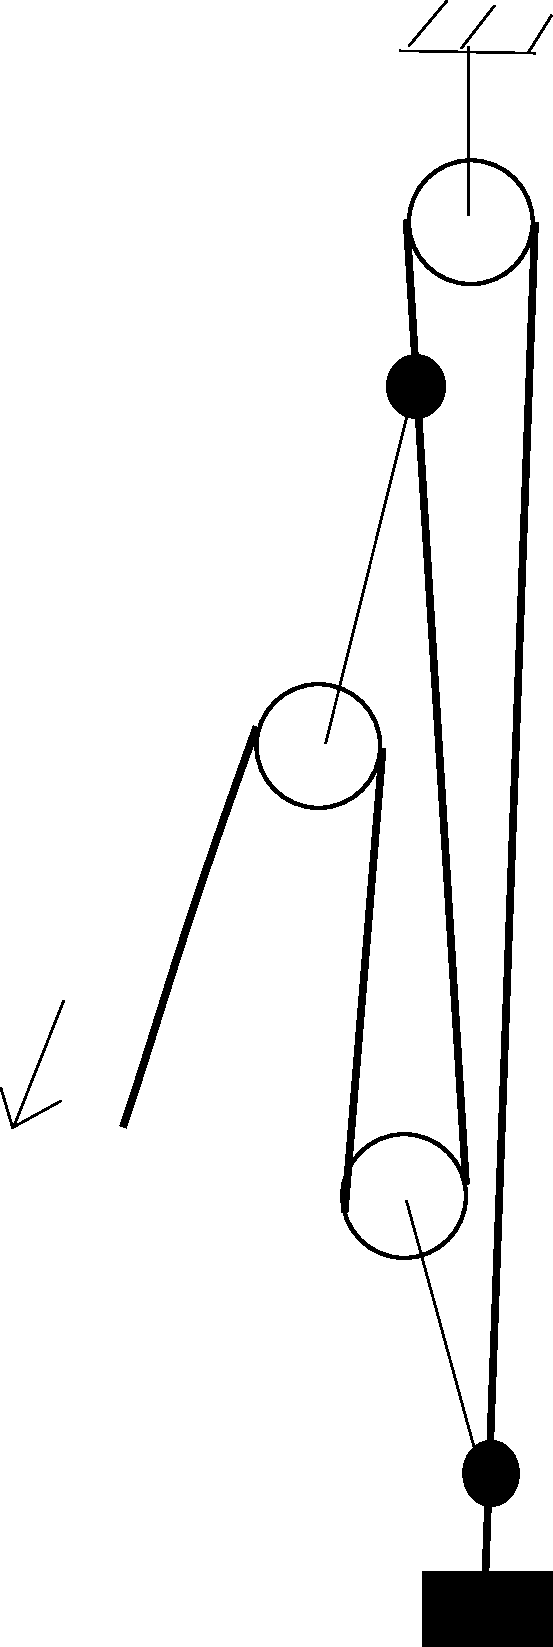
\includegraphics[width=0.25\linewidth]{2014-v3g-06-Polyspast}
\end{center}
\fi


\ifEngHint
In the case of a frictionless block the tension in the main rope is permanent, only its direction changes. In addition, to satisfy equilibrium conditions the tension of the block’s attachment has to be equal to the sum of the main’s rope tensions going through the block. It is convenient to start solving the problem from the savior’s position and assume that the corresponding attractive force is $F$.
\fi


\ifEngSolution
For a frictionless block the tension in the main rope is constant, only its direction changes. In the case of a block with friction a part of the main rope’s tension is transmitted to the block, moreover in the first approximation downwards and upwards directed frictions compensate each other. To satisfy the equilibrium condition the block’s attachment tension has to be equal to sum of the main rope’s tensions that go through the block. In the case of non-sliding knots the upwards and downwards directed tensions have to be in balance. It is easy to start solving if you assume the force from the rescuer’s side to be $F$ and begin by going through the polyspast from the rescuer’s end. In the frictionless case the force transmission is $\frac{5}{1}$ and in the case of friction $\frac{2,4}{1}$. 
\begin{center}
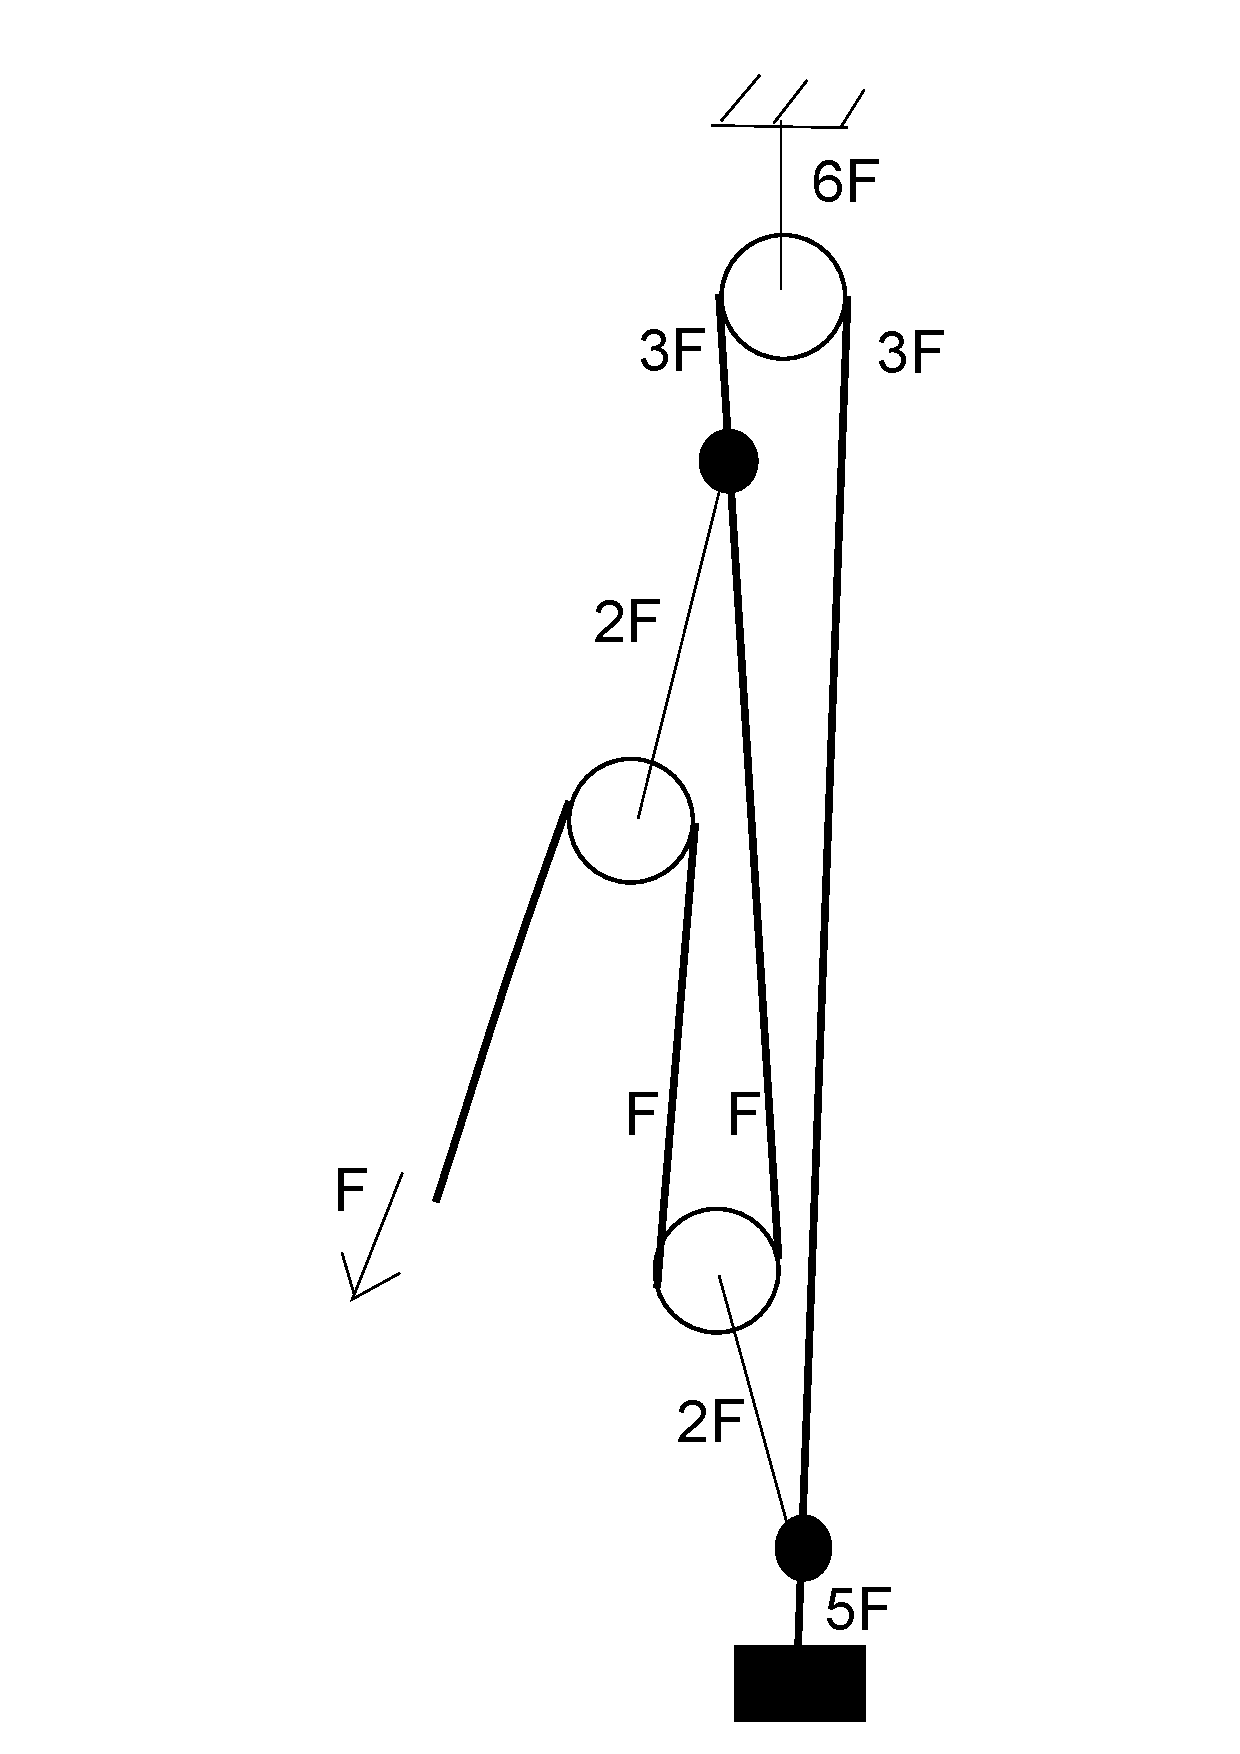
\includegraphics[scale=0.25]{2014-v3g-06-PolyspastL1}
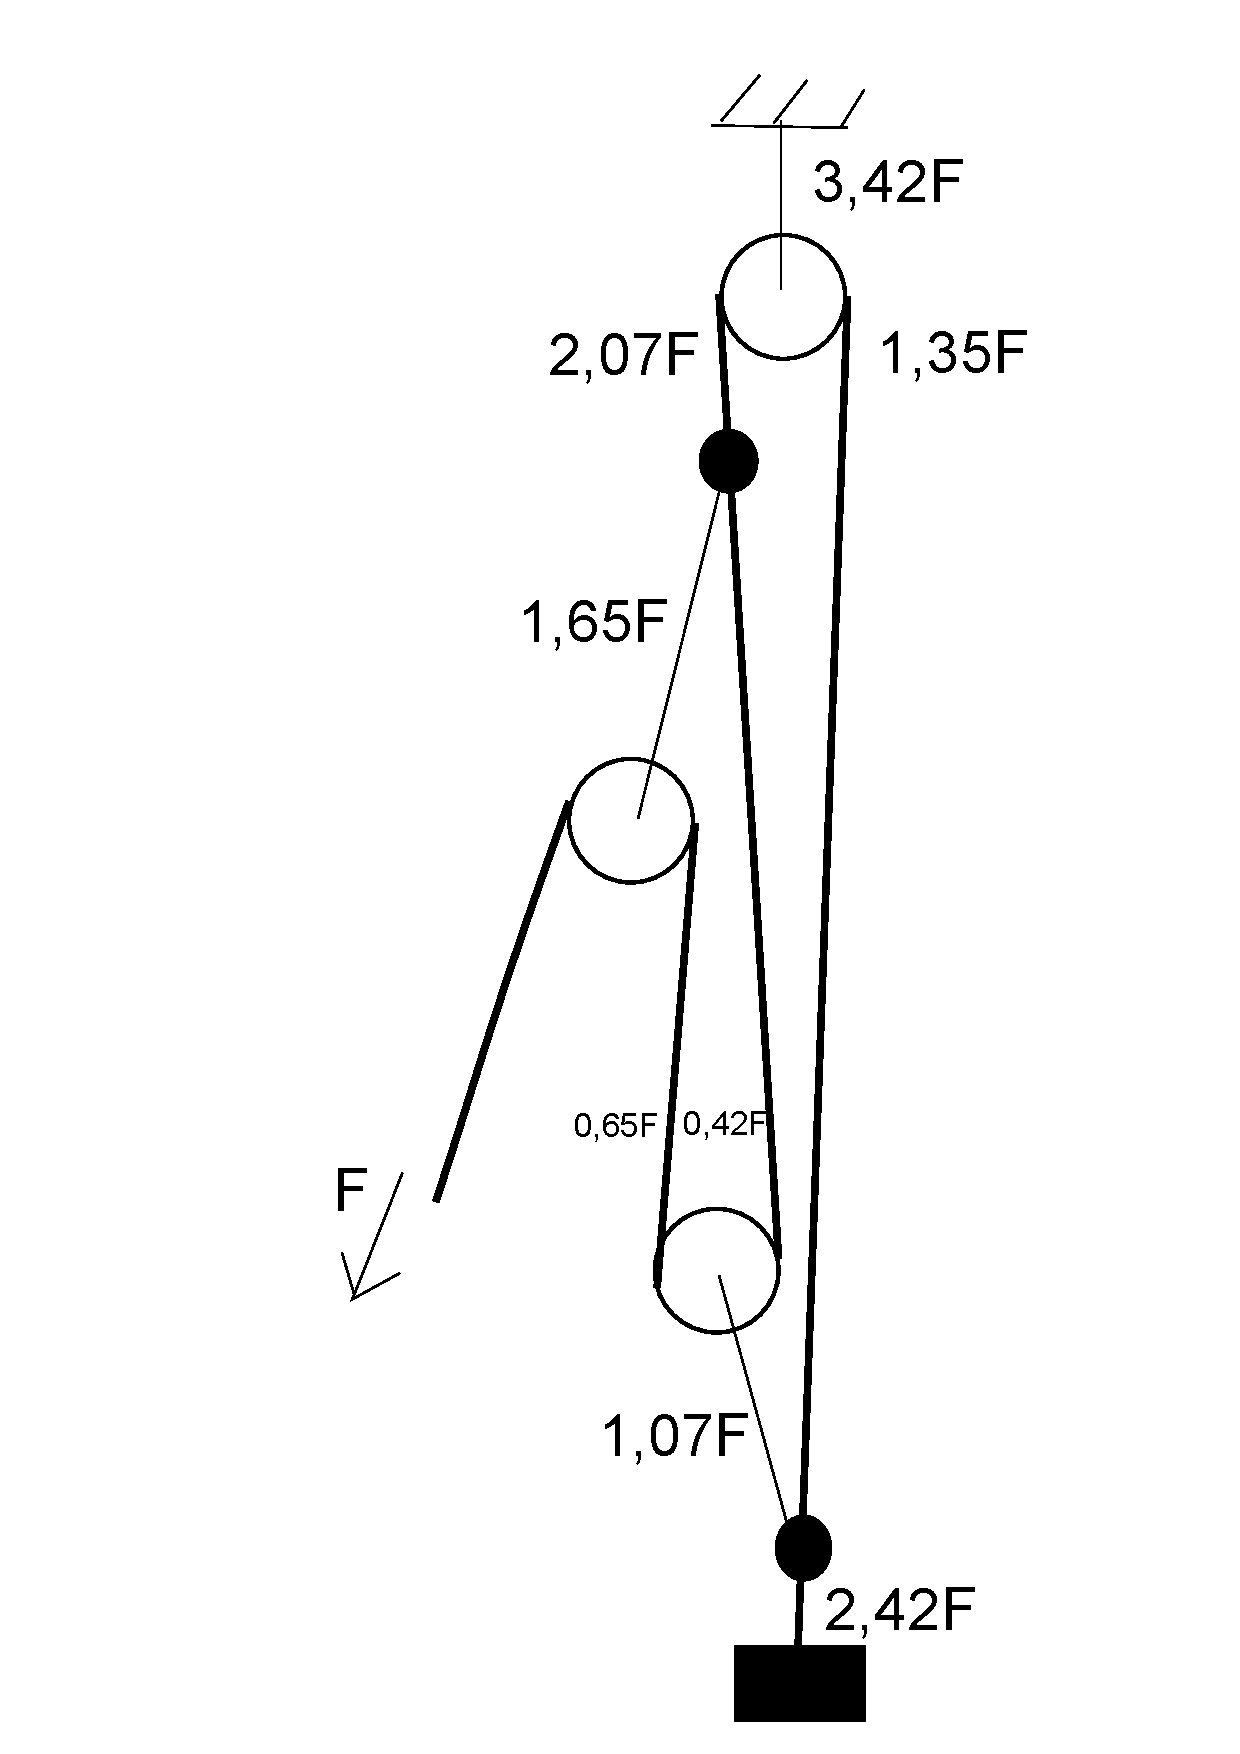
\includegraphics[scale=0.25]{2014-v3g-06-PolyspastL2}
\end{center}
\fi
}